
\documentclass{report}

\usepackage[utf8]{inputenc}
\usepackage[italian]{babel}
\usepackage{import}
\usepackage{todonotes}
\usepackage{color}
\usepackage{rotating}
\usepackage[hidelinks]{hyperref}
\usepackage{url}
\usepackage{pdfpages}
\usepackage{siunitx}
\usepackage{pdflscape}
\usepackage{subfig}
\usepackage[euler]{textgreek}
\usepackage{mhchem}

\usepackage{multirow}

\usepackage{enumerate} 
\usepackage{amsmath}
\usepackage{amsfonts}

\usepackage[signatures,swapnames,sans]{frontespizio}

\usepackage{geometry}
\geometry{portrait, margin=3cm}
\usepackage{siunitx}
\usepackage{booktabs}

\renewcommand*\figurename{Figura}

\newcommand{\sub}[1]{\textsubscript{#1}}
\newcommand{\super}[1]{\textsuperscript{#1}}
\newcommand{\parallelsum}{\mathbin{\!/\mkern-5mu/\!}}

\newcommand{\Fig}[0]{Fig.}

\usepackage{titlesec}

\titleformat{\chapter}{\normalfont\huge}{}{20pt}{\huge\bfseries}

\linespread{1.3}


%% COMANDI UTILI
%\begin{table}[h]
%	\centering
%	\begin{tabular}{|c|c|c|}
%	\cline{2-3} 
%	\multicolumn{1}{c|}{} & \textbf{Valore nominale} & \textbf{Valore misurato}\\ 
%		%\hline
%		%{} & \textbf{Valore nominale} & \textbf{Valore misurato} \\ 
%		\hline
%		$\mathbf{R_1}$ & \SI{18}{k\ohm} & \SI{17.977}{k\ohm} \\ 
%		\hline
%		$\mathbf{R_2}$& \SI{1.8}{k\ohm} & \SI{1.815}{k\ohm} \\ 
%		\hline
%	\end{tabular}
%\caption{Misure delle resistenze utilizzate per il circuito.}
%\label{table:mis_res}
%\end{table}
%\begin{figure}[h!]
%\centering
%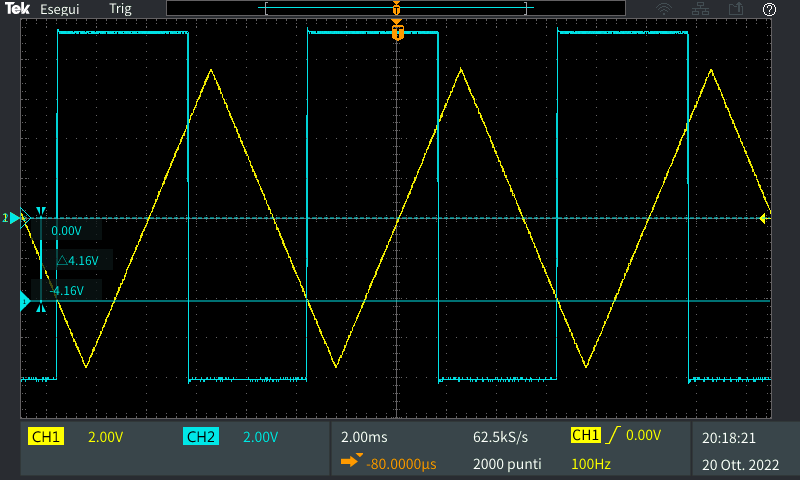
\includegraphics[height=6.5cm]{immagini/TEK00018}\\(a)\\[1ex]
%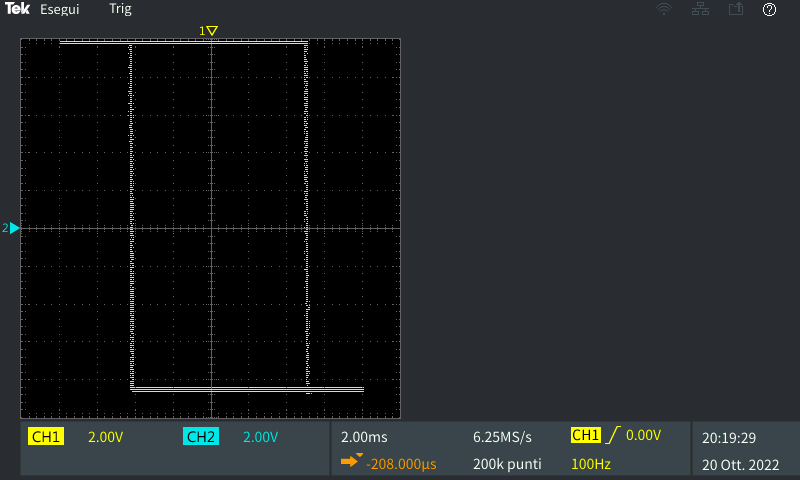
\includegraphics[height=6.5cm]{immagini/TEK00019}\\(b)
%\caption{Risposta del circuito con accoppiamento DC (a) e accoppiamento AC (b).}
%	\label{figura:accopp}
%\end{figure}

\begin{document}
\addtocounter{chapter}{+2}
	\begin{frontespizio}
		\Margini{3cm}{3cm}{3cm}{3cm}
		\Universita{Bergamo}
		\Logo[43.332mm]{unibg-mark}
		\Divisione{Scuola di Ingegneria}
		\Corso[Laurea Magistrale]{Ingegneria Informatica}
		\Titolo{Laboratorio di Elettronica}
		\Sottotitolo{Relazione esperienza di laboratorio 3}
		\Punteggiatura{}
		\NRelatore{Prof.}{Prof.}
		\Relatore{Luigi Gaioni}
		\Candidato[1058231]{Giulia Allievi}
		\Candidato[1059640]{Martina Fanton}
		\Annoaccademico{2022--2023}
		\begin{Preambolo*}
			\usepackage[italian]{babel}
			\usepackage[T1]{fontenc}
			\usepackage[utf8]{inputenc}
			\usepackage{microtype}
			\usepackage{lmodern}
			\graphicspath{{img/}}
			
			\renewcommand{\frontinstitutionfont}{\fontsize{14}{17}\bfseries\scshape}
			\renewcommand{\fronttitlefont}{\fontsize{17}{21}\bfseries\scshape}
			\renewcommand{\frontfootfont}{\fontsize{12}{14}\bfseries\scshape}
		\end{Preambolo*}
	\end{frontespizio}

%----------------------------------------------------------------------------------------
%	PAGINA BIANCA
%----------------------------------------------------------------------------------------
\newpage
\null
\thispagestyle{empty}
\newpage

%----------------------------------------------------------------------------------------
%	INTRO
%----------------------------------------------------------------------------------------
\chapter{Relazione attività di laboratorio 3}
\section*{Introduzione}
In questo laboratorio, sono stati analizzati circuiti composti da diodi e/o da amplificatori operazionali.
In particolare il primo circuito analizzato permette di risolvere un problema che si verificava nell'ultimo circuito analizzato durante il precedente laboratorio, ovvero nel raddrizzatore a doppia semionda. Questo problema consisteva nella presenza di una differenza di tensione, idealmente pari a \SI{0.7}{\volt} (mentre nelle nostre misure risultava pari a \SI{0.460}{\volt}), tra il segnale in uscita e quello in ingresso.
\\Il secondo circuito invece è un trigger di  Schmitt, che presenta nella sua caratteristica tra la tensione di ingresso e quella di uscita un ciclo di isteresi.
\\Infine il terzo circuito e il quarto funzionano senza la necessità di applicare un segnale in ingresso.
% DA SISTEMARE

\newpage
\section{Circuito 1: raddrizzatore a doppia semionda di precisione}
\subsection{Schema del circuito e Funzione di Trasferimento}
Questo circuito, come si può notare dalla figura \ref{figura:schema1}, presenta due amplificatori operazionali, di cui quello in alto è retroazionato negativamente, e un diodo.
\begin{figure}[h]
	\centering
	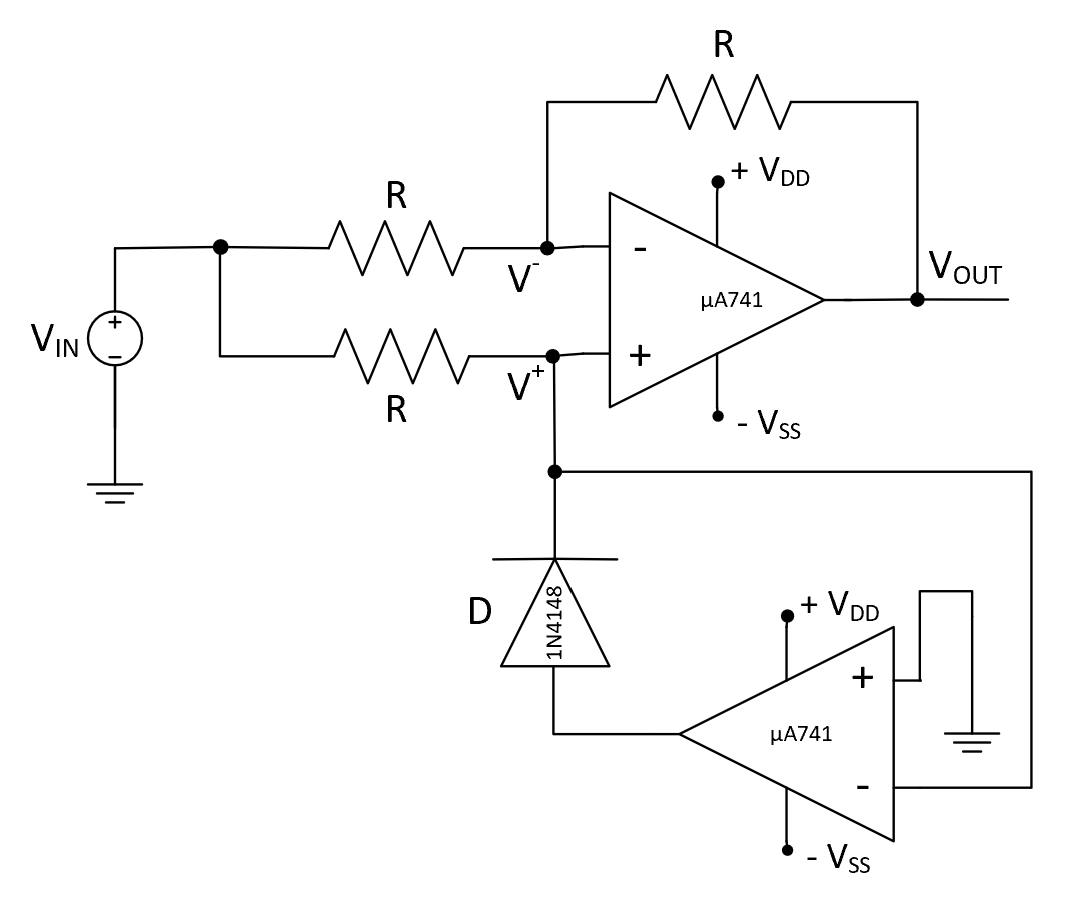
\includegraphics[height=6.2cm]{immagini/schema1}
	\caption{Schema del raddrizzatore a doppia semionda di precisione.}
	\label{figura:schema1}
\end{figure}
\\ \noindent La funzione di trasferimento di questo raddrizzatore è:
\begin{equation}
   \begin{cases}
   V_{in}< \SI{0}{\volt}\;\;\indent\indent\rightarrow \mathrm{D\;ON}\;\;\;\; \Rightarrow V_{out} = -V_{in}\\
   V_{in}\ge \SI{0}{\volt}\;\;\indent\indent\rightarrow \mathrm{D\; OFF}\;\; \Rightarrow V_{out} = V_{in}
   \end{cases}
\end{equation}
Da questa Funzione di Trasferimento si può notare che l'uscita non risulta shiftata rispetto all'uscita, come invece succedeva nel raddrizzatore a doppia semionda analizzato durante lo scorso laboratorio. Dunque questo circuito permette di risolvere il problema della differenza di tensione presente tra uscita e ingresso.
\\Di conseguenza in uscita si ottiene un segnale analogo a quello in ingresso, ma in cui le semionde risultano raddrizzate.
\subsection{Analisi e dati sperimentali}
Per la realizzazione del circuito sulla breadboard (visibile nella figura \ref{figura:circuito1}) abbiamo deciso di utilizzare due amplificatori operazionali di tipo \textmu A741, che sono amplificatori operazionali \textit{general purpose}, e un diodo di tipo 1N4148.
Invece per quanto riguarda i valori delle resistenze abbiamo utilizzato resistenze da \SI{12}{k\ohm}, le cui misure sono state riportate nella tabella \ref{table:mis_res1}.
\begin{table}[h!]
	\centering
	\begin{tabular}{|c|c|c|}
		\cline{2-3} 
		\multicolumn{1}{c|}{} & \textbf{Valore nominale} & \textbf{Valore misurato}\\ 
		\hline
		$\mathbf{R_1}$ & \SI{12}{k\ohm} & \SI{11.802}{k\ohm} \\ 
		\hline
		$\mathbf{R_2}$ & \SI{12}{k\ohm} & \SI{11.947}{k\ohm} \\ 
		\hline
		$\mathbf{R_3}$ & \SI{12}{k\ohm} & \SI{11.885}{k\ohm} \\ 
		\hline
	\end{tabular}
	\caption{Misure delle resistenze utilizzate per il circuito.}
	\label{table:mis_res1}
\end{table}
\begin{figure}[h]
	\centering
	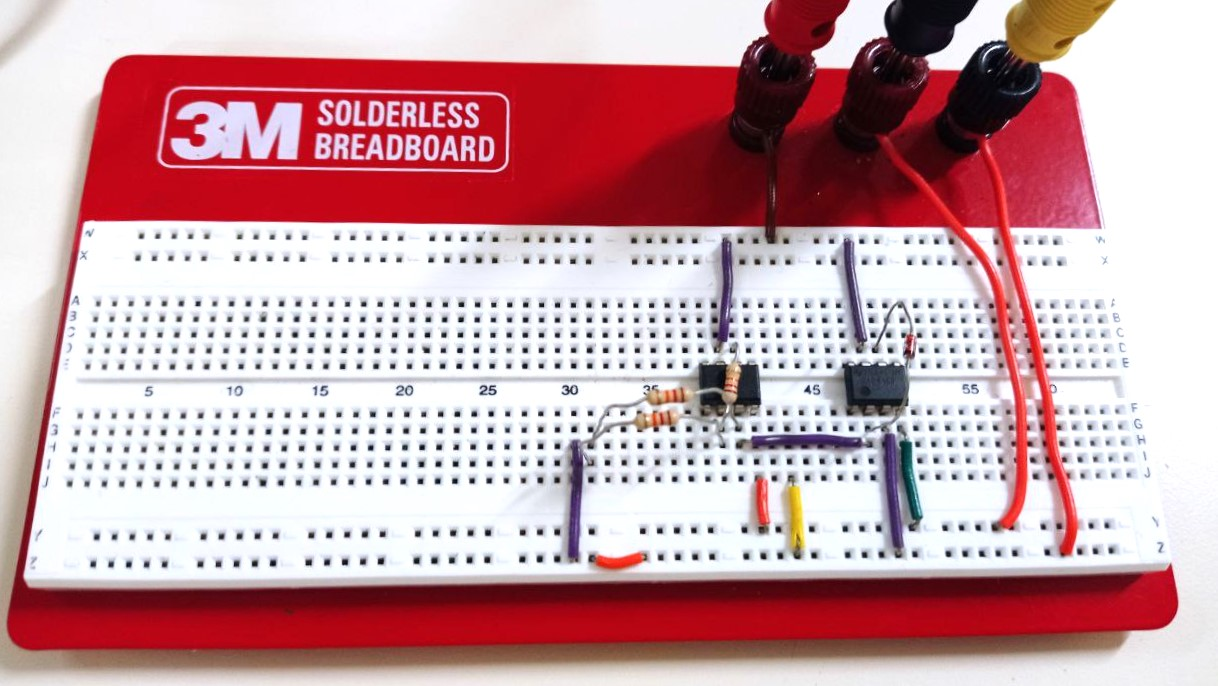
\includegraphics[height=6.2cm]{immagini/circuito1}
	\caption{Fotografia del raddrizzatore a doppia semionda di precisione realizzato in laboratorio.}
	\label{figura:circuito1}
\end{figure}
\\\\\\
\\Dopo aver realizzato il circuito sulla breadboard, sono stati collegati sia la alimentazioni (con un valore di \SI{+10}{\volt}) e di \SI{-10}{\volt} sia il segnale d'ingresso (con un'ampiezza picco-picco di \SI{2}{\volt}).
\\Il segnale in uscita prodotto dall'oscilloscopio lo si può vedere nelle figure \ref{figura:uscita11} per frequenze pari a \SI{100}{\hertz} e a \SI{1}{k\hertz}. Per queste frequenze sono state analizzate anche le rappresentazioni XY (in figure \ref{figura:xyuscita1}), ovvero le caratteristiche tra tensione di ingresso e tensione di uscita del circuito.
\begin{figure}[h!]
	\centering
	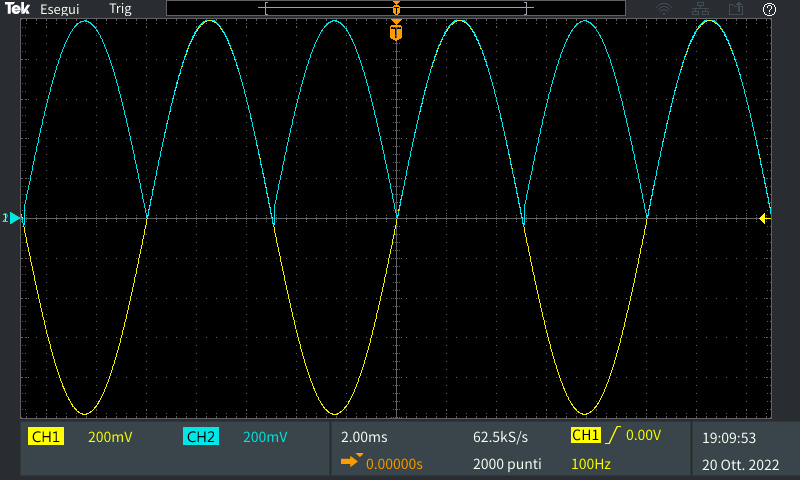
\includegraphics[height=4.6cm]{immagini/TEK00000}
	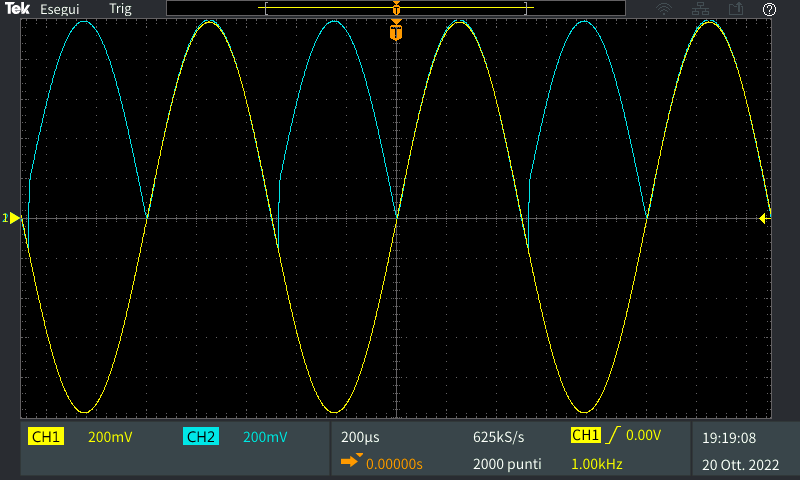
\includegraphics[height=4.6cm]{immagini/TEK00003}
	\caption{Risposta del circuito con $\mathrm{f= \SI{100}{\hertz}}$ (sinistra) e con $\mathrm{f= \SI{1}{k\hertz}}$ (destra).}
	\label{figura:uscita11}
\end{figure}
\begin{figure}[h!]
	\centering
	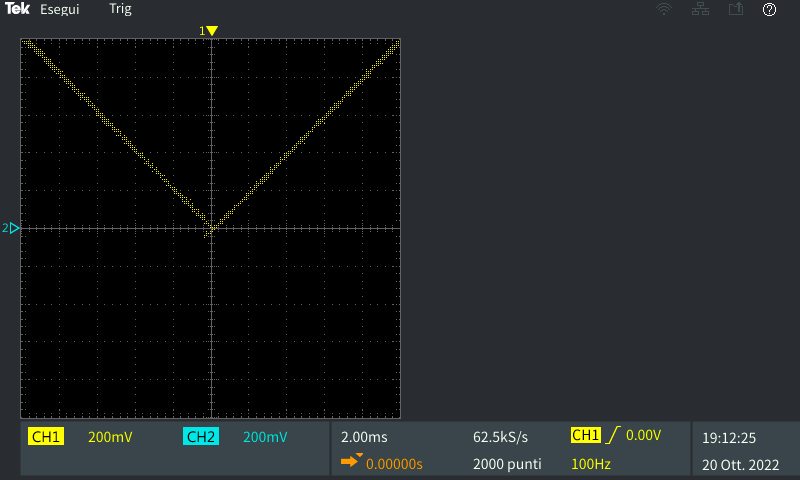
\includegraphics[height=4.6cm]{immagini/TEK00001}
	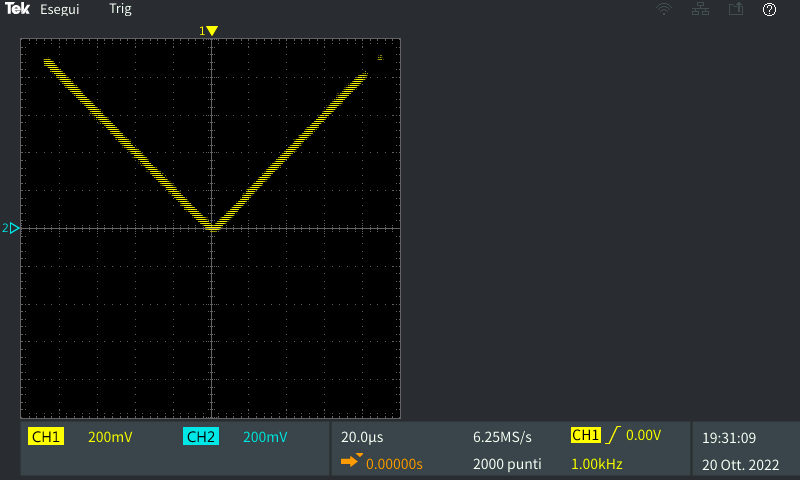
\includegraphics[height=4.6cm]{immagini/TEK00010}
	\caption{Rappresentazione XY della risposta del circuito con $\mathrm{f= \SI{100}{\hertz}}$ (sinistra) e con $\mathrm{f= \SI{1}{k\hertz}}$ (destra).}
	\label{figura:xyuscita1}
\end{figure}
\\\\\\
\\In tutti questi grafici il segnale presenta un andamento quasi ideale, ma nella parte iniziale delle semionde negative raddrizzate si possono notare dei tratti anomali vicino all'asse delle ascisse. Queste anomalie sono dovute al fatto che l'OPAMP in basso può avere una retroazione aperta per la presenza del diodo e quindi la sua uscita deve svolgere uno swing abbastanza ampio (visualizzato nelle figure \ref{figura:uscita111}) per far arrivare la sua uscita al valore dell'alimentazione. Questo poi incide anche sulla velocità del sistema.
\begin{figure}[h!]
	\centering
	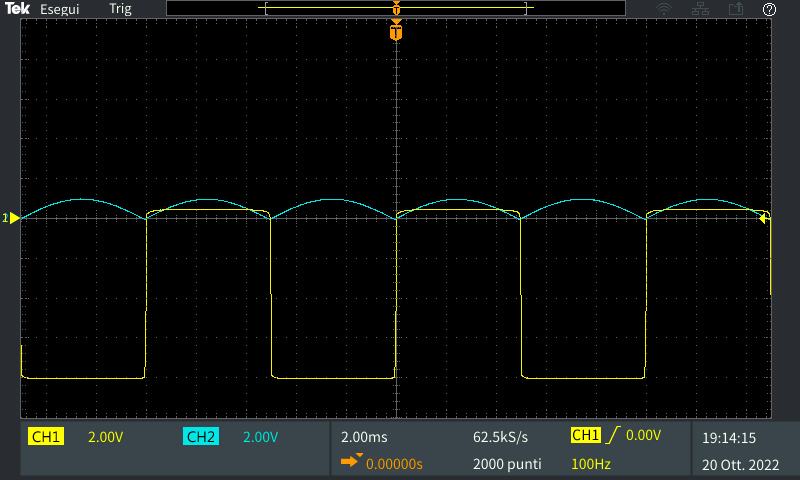
\includegraphics[height=4.6cm]{immagini/TEK00002}
	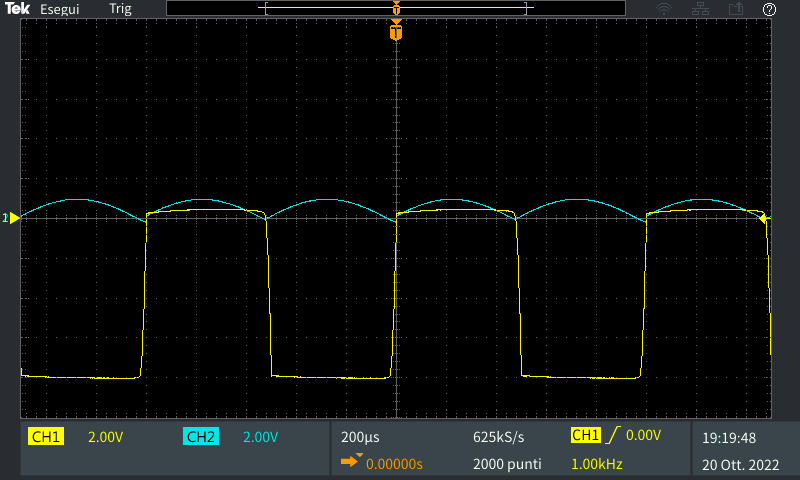
\includegraphics[height=4.6cm]{immagini/TEK00004}
	\caption{Risposta dell'OPAMP in basso con $\mathrm{f= \SI{100}{\hertz}}$ (sinistra) e con $\mathrm{f= \SI{1}{k\hertz}}$ (destra).}
	\label{figura:uscita111}
\end{figure}
\\Analizzando invece frequenze maggiori (ad esempio \SI{10}{k\hertz}), il segnale presenta delle anomalie di maggiore rilevanza rispetto alle precedenti come si può notare nella figura \ref{figura:uscita12}. Tutte queste anomalie derivano dal fatto che l'OPAMP non è adatto a operare in alta frequenza quando presenta un anello che può risultare aperto.
\begin{figure}[h!]
	\centering
	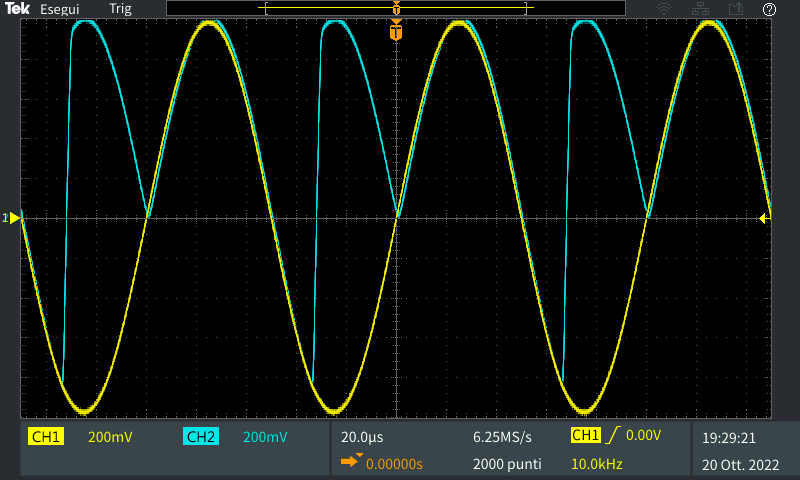
\includegraphics[height=4.6cm]{immagini/TEK00008}
	\caption{Risposta del circuito con $\mathrm{f= \SI{10}{k\hertz}}$.}
	\label{figura:uscita12}
\end{figure}

\newpage
\section{Circuito 2: trigger di Schmitt}
\subsection{Schema del circuito e Funzione di Trasferimento}
In questo circuito è presente un amplificatore operazionale non retroazionato negativamente, ma con una retroazione positiva e quindi il circuito opera come un comparatore.
\\Inoltre è costituito anche da una rete sulla retroazione formata da un partitore resistivo, in cui le due resistenze sono equivalenti.
\\La caratteristica principale di questo circuito è che, a differenza dei normali comparatori, presenta in uscita un'isteresi. Inoltre questo circuito è immune a eventuali disturbi presenti sui possibili segnali in ingresso perchè in un comparatore se il segnale in ingresso è rumoroso su valori prossimi alla soglia ${V^+}$ si possono avere delle transizioni involontarie dell'uscita da ${V_{DD}}$ a ${V_{SS}}$. Questo problema viene infatti risolto nel trigger di Schmitt perchè una volta attraversata la soglia quest'ultima varierà il suo valore e quindi andrebbe attraversata la nuova soglia per avere un'ulteriore transizione.
\begin{figure}[h]
	\centering
	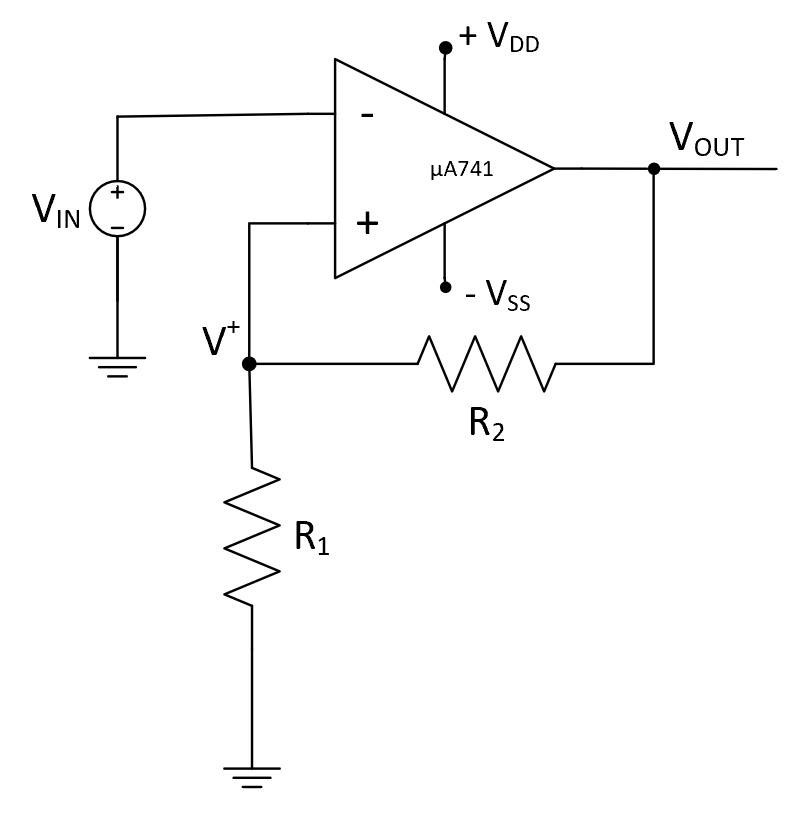
\includegraphics[height=6.2cm]{immagini/schema2}
	\caption{Schema del trigger di Schmitt.}
	\label{figura:schema2}
\end{figure}
\\ \noindent La funzione di trasferimento di questo comparatore è:
\begin{equation}
   \begin{cases} % da controllare
   V_{out}= V_{DD}\;\indent\indent \mathrm{per\;}  V_L^+<V_{in}<V_H^+\mathrm{, \;\; con\;}\displaystyle{ V_H^+=\frac{R_1}{R_1+R_2}\cdot V_{DD}=\frac{V_{DD}}{2}}\mathrm{\;\;\;\; se \;} R_1=R_2\\[10pt]
   V_{out}= V_{SS}\;\;\indent\indent \mathrm{per\;} V_H^+<V_{in}<V_L^+\mathrm{, \;\; con\;}\displaystyle{ V_H^+=\frac{R_1}{R_1+R_2}\cdot |V_{SS}|=\frac{|V_{SS}|}{2}}\mathrm{\;\; se \;} R_1=R_2\\
   \end{cases}
\end{equation}
% SISTEMARE FDT
%\begin{equation}
%	\begin{cases} % da controllare
%		V_{out}= V_{DD}\;\indent\indent \mathrm{per\; t\; da\;} V_{in}=V_L^+\mathrm{\; a\;}V_{in}=V_H^+\mathrm{, \;\; con\;}\displaystyle{ V_H^+=\frac{R_1}{R_1+R_2}\cdot V_{DD}=\frac{V_{DD}}{2}}\mathrm{\;\;\;\; se \;} R_1=R_2\\[10pt]
%		V_{out}= V_{SS}\;\;\indent\indent \mathrm{per\; t\; da\;} V_{in}=V_H^+\mathrm{\; a\;}V_{in}=V_L^+\mathrm{, \;\; con\;}\displaystyle{ V_H^+=\frac{R_1}{R_1+R_2}\cdot |V_{SS}|=\frac{|V_{SS}|}{2}}\mathrm{\;\; se \;} R_1=R_2\\
%	\end{cases}
%\end{equation}
\subsection{Analisi e dati sperimentali}
Per la realizzazione del circuito sulla breadboard (visibile nella figura \ref{figura:circuito2}) è stato utilizzato un amplificatore operazionale di tipo \textmu A741.
Invece per quanto riguarda i valori delle resistenze abbiamo utilizzato due resistenze da \SI{12}{k\ohm}, le cui misure sono state riportate nella tabella \ref{table:mis_res2}.
\begin{table}[h!]
	\centering
	\begin{tabular}{|c|c|c|}
		\cline{2-3} 
		\multicolumn{1}{c|}{} & \textbf{Valore nominale} & \textbf{Valore misurato}\\ 
		\hline
		$\mathbf{R_1}$ & \SI{12}{k\ohm} & \SI{11.802}{k\ohm} \\ 
		\hline
		$\mathbf{R_2}$ & \SI{12}{k\ohm} & \SI{11.947}{k\ohm} \\ 
		\hline
	\end{tabular}
	\caption{Misure delle resistenze utilizzate per il circuito.}
	\label{table:mis_res2}
\end{table}
\begin{figure}[h]
	\centering
	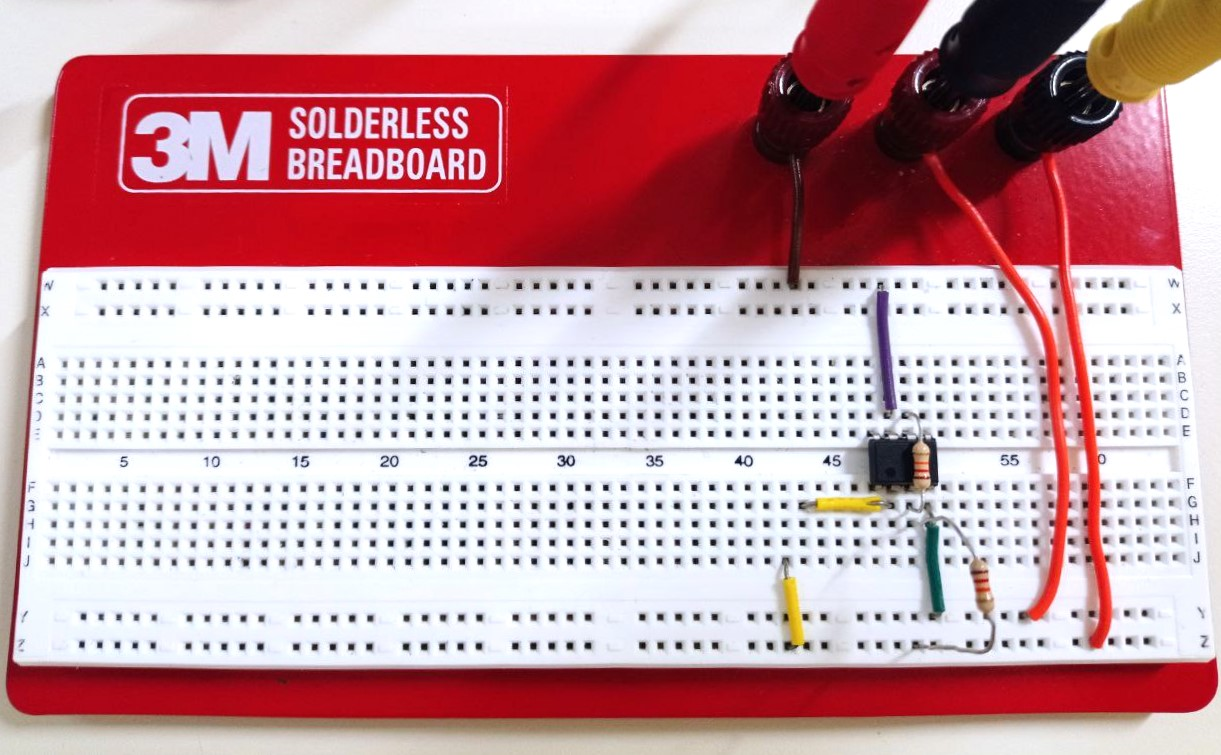
\includegraphics[height=6.2cm]{immagini/circuito2}
	\caption{Fotografia del trigger di Schmitt realizzato in laboratorio.}
	\label{figura:circuito2}
\end{figure}
\\Dopo aver realizzato la breadboard, come segnale in ingresso è stata utilizzata un'onda triangolare con ampiezza picco-picco di \SI{15}{\volt}.
\\Per prima cosa abbiamo analizzato l'uscita del circuito con un segnale in ingresso con frequenza di \SI{100}{\hertz} (figure \ref{figura:uscita21}).
\begin{figure}[h!]
	\centering
	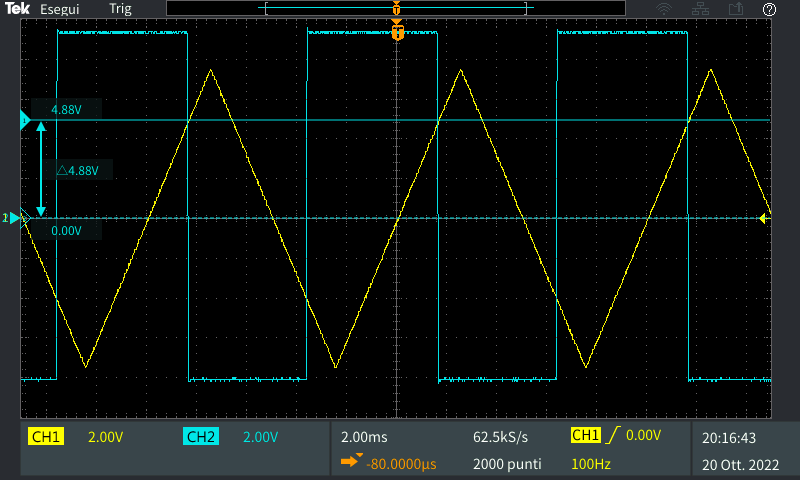
\includegraphics[height=4.6cm]{immagini/TEK00017}
	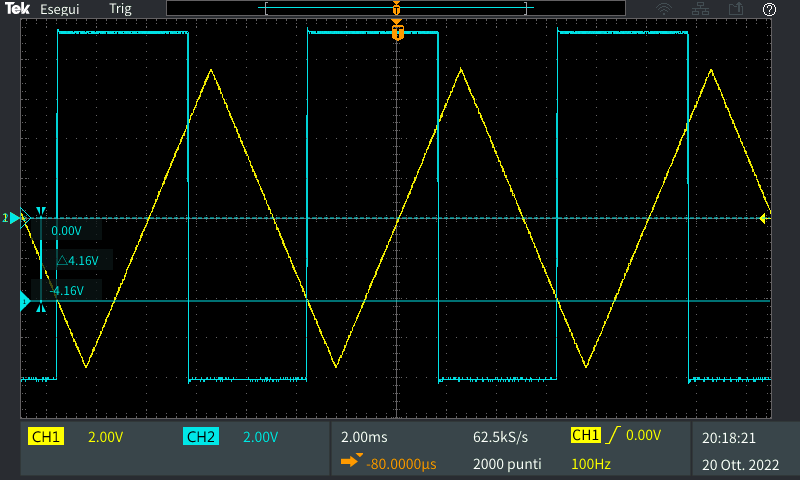
\includegraphics[height=4.6cm]{immagini/TEK00018}
	\caption{Risposta del circuito con $\mathrm{f= \SI{100}{\hertz}}$.}
	\label{figura:uscita21}
\end{figure}
\\\\\\\\\\
\\Dai grafici si può notare che il comportamento dei segnali risulta corretto e poi sono state misurate le due soglie, i cui valori sono risultati pari a \SI{4.88}{\volt} per ${V_H^+}$ (soglia positiva) e \SI{-4.16}{\volt} per ${V_L^+}$ (soglia negativa).
\\Successivamente è stato analizzato anche il grafico della caratteristica ingresso-uscita per la stessa frequenza. Come si può notare dalla figura \ref{figura:uscita22}, è presente un ciclo di isteresi, come ci si aspettava per questo trigger.
\begin{figure}[h!]
	\centering
	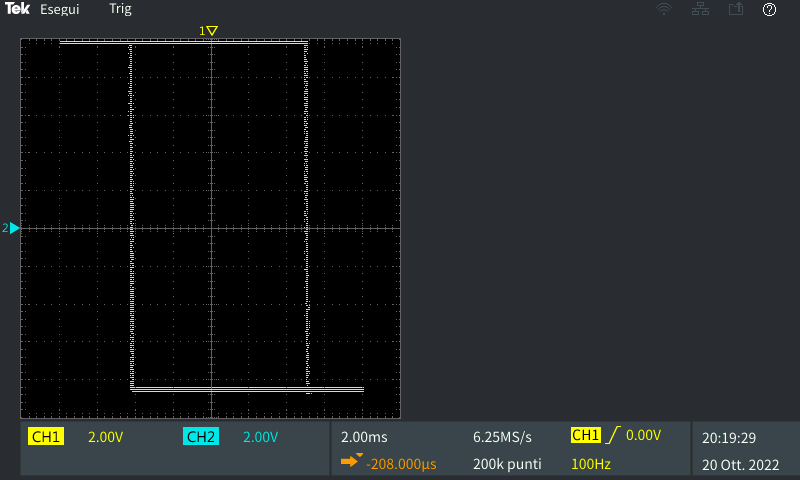
\includegraphics[height=4.6cm]{immagini/TEK00019}
	\caption{Rappresentazione XY della risposta del circuito con $\mathrm{f= \SI{100}{\hertz}}$.}
	\label{figura:uscita22}
\end{figure}

\newpage
\section{Circuito 3: oscillatore con duty cicle = 50\%}
\subsection{Schema del circuito e Funzione di Trasferimento}
\begin{figure}[h]
	\centering
	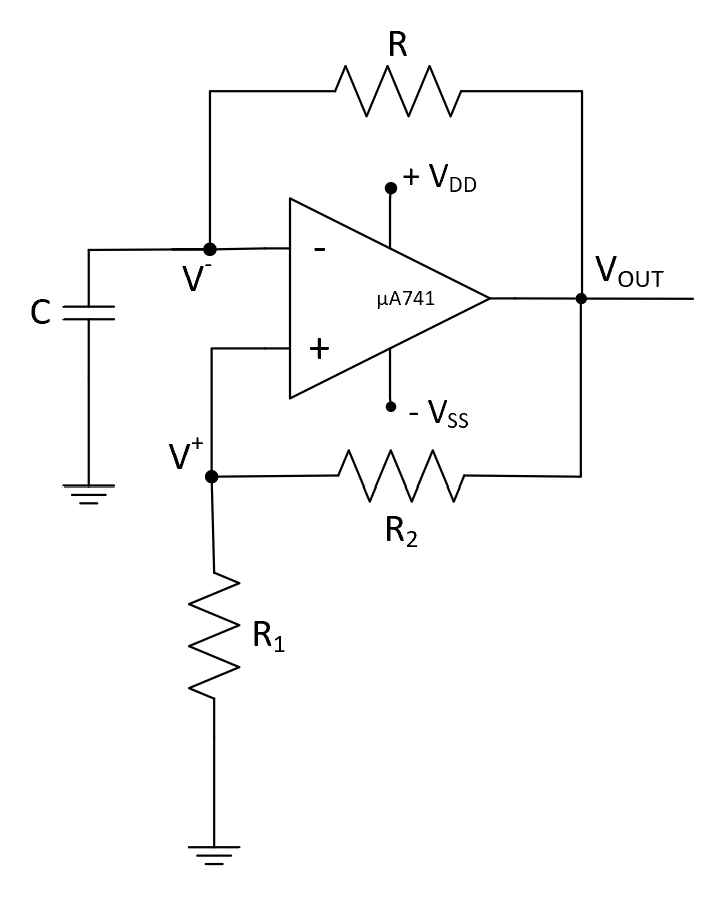
\includegraphics[height=6.2cm]{immagini/schema3}
	\caption{Schema dell'oscillatore con duty cicle = 50\%.}
	\label{figura:schema3}
\end{figure}
%\noindent La funzione di trasferimento di questo raddrizzatore è:
%\begin{equation}
%   \begin{cases}
	%   \end{cases}
%\end{equation}
\subsection{Analisi e dati sperimentali}
\begin{figure}[h]
	\centering
	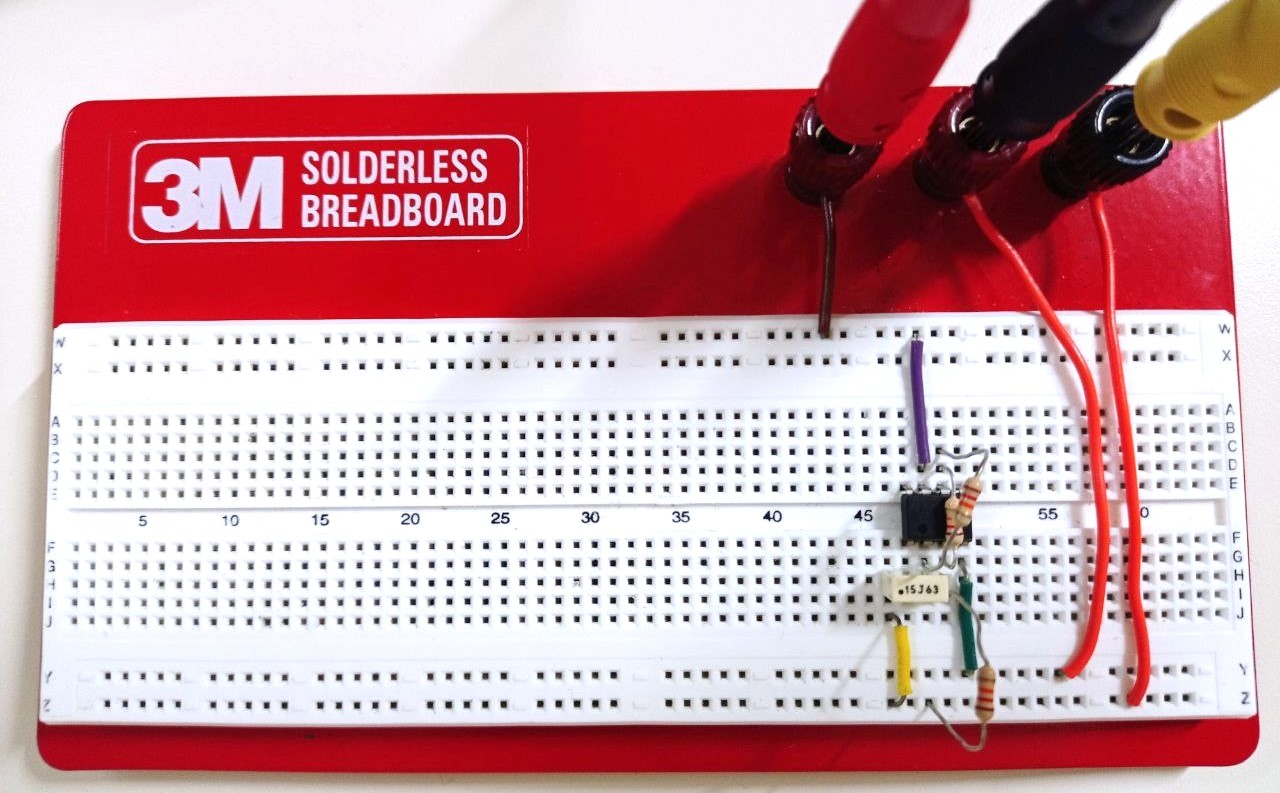
\includegraphics[height=6.2cm]{immagini/circuito3}
	\caption{Fotografia dell'oscillatore con duty cicle = 50\% realizzato in laboratorio.}
	\label{figura:circuito3}
\end{figure}
%\begin{table}[h!]
%	\centering
%	\begin{tabular}{|c|c|c|}
	%		\cline{2-3} 
	%		\multicolumn{1}{c|}{} & \textbf{Valore nominale} & \textbf{Valore misurato}\\ 
	%		\hline
	%		$\mathbf{R_1}$ & \SI{18}{k\ohm} & \SI{17.977}{k\ohm} \\ 
	%		\hline
	%		$\mathbf{R_2}$ & \SI{33}{k\ohm} & \SI{37.630}{k\ohm} \\ 
	%		\hline
	%		$\mathbf{R_3}$ & \SI{56}{k\ohm} & \SI{54.742}{k\ohm} \\ 
	%		\hline
	%		$\mathbf{R_4}$ & $\displaystyle\mathrm{\SI{82}{k\ohm}+\SI{18}{k\ohm}=\SI{100}{k\ohm}}$ & $\displaystyle\mathrm{\SI{80.717}{k\ohm+}\SI{17.977}{k\ohm}=\SI{98.694}{k\ohm}}$ \\ 
	%		\hline
	%	\end{tabular}
%	\caption{Misure delle resistenze utilizzate nel raddrizzatore a semionda passivo.}
%	\label{table:misure1}
%\end{table}

\section{Circuito 4: oscillatore con duty cicle $\neq$ 50\%}
\subsection{Schema del circuito e Funzione di Trasferimento}
\begin{figure}[h]
	\centering
	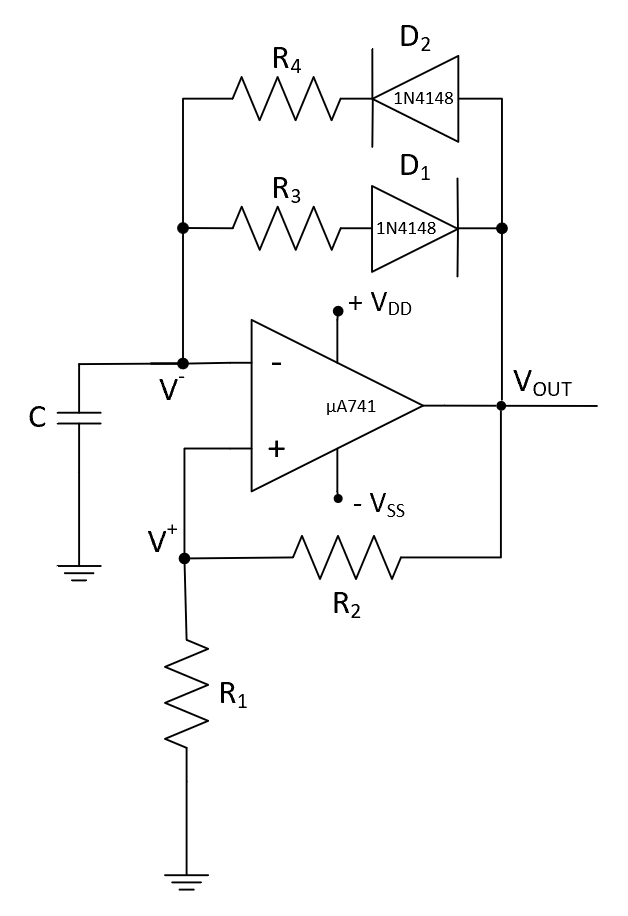
\includegraphics[height=6.2cm]{immagini/schema4}
	\caption{Schema dell'oscillatore con duty cicle $\neq$ 50\%.}
	\label{figura:schema4}
\end{figure}
%\noindent La funzione di trasferimento di questo raddrizzatore è:
%\begin{equation}
%   \begin{cases}
	%   \end{cases}
%\end{equation}
\subsection{Analisi e dati sperimentali}
\begin{figure}[h]
	\centering
	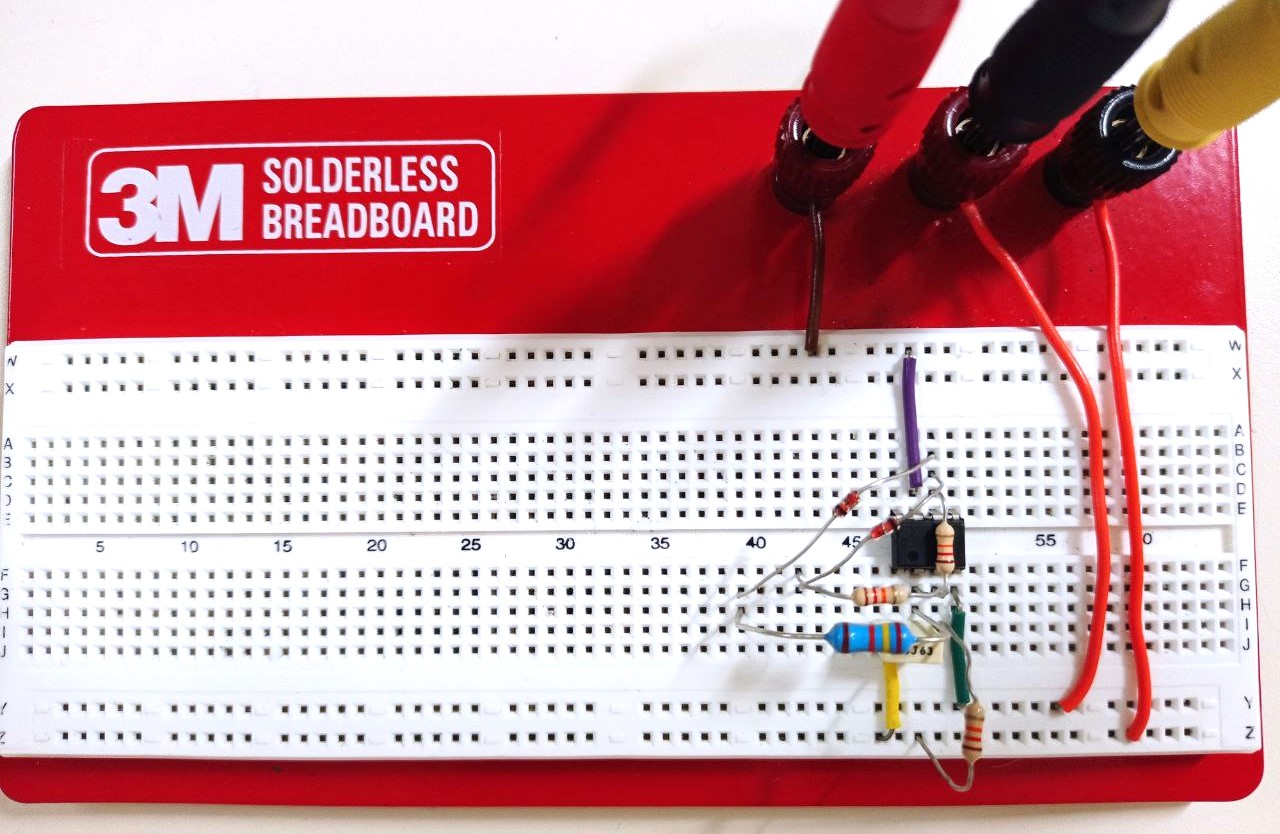
\includegraphics[height=6.2cm]{immagini/circuito4_1.jpg}
	\caption{Fotografia dell'oscillatore con duty cicle $\neq$ 50\% realizzato in laboratorio.}
	\label{figura:circuito4}
\end{figure}
%\begin{table}[h!]
%	\centering
%	\begin{tabular}{|c|c|c|}
	%		\cline{2-3} 
	%		\multicolumn{1}{c|}{} & \textbf{Valore nominale} & \textbf{Valore misurato}\\ 
	%		\hline
	%		$\mathbf{R_1}$ & \SI{18}{k\ohm} & \SI{17.977}{k\ohm} \\ 
	%		\hline
	%		$\mathbf{R_2}$ & \SI{33}{k\ohm} & \SI{37.630}{k\ohm} \\ 
	%		\hline
	%		$\mathbf{R_3}$ & \SI{56}{k\ohm} & \SI{54.742}{k\ohm} \\ 
	%		\hline
	%		$\mathbf{R_4}$ & $\displaystyle\mathrm{\SI{82}{k\ohm}+\SI{18}{k\ohm}=\SI{100}{k\ohm}}$ & $\displaystyle\mathrm{\SI{80.717}{k\ohm+}\SI{17.977}{k\ohm}=\SI{98.694}{k\ohm}}$ \\ 
	%		\hline
	%	\end{tabular}
%	\caption{Misure delle resistenze utilizzate nel raddrizzatore a semionda passivo.}
%	\label{table:misure1}
%\end{table}

%----------------------------------------------------------------------------------------

\end{document}
